\documentclass[border=2pt]{standalone}
\usepackage{fontspec}
\setmainfont{Liberation Serif}
\usepackage{tikz,graphicx,pgfplots}
\usetikzlibrary{arrows.meta,positioning,matrix,calc}
\pgfplotsset{compat=1.18}
\definecolor{forest}{HTML}{176044}
\definecolor{sage}{HTML}{EAF4EE}
\definecolor{rulec}{HTML}{CBD4CF}
\definecolor{ink}{HTML}{192723}
\definecolor{warm}{HTML}{F3ECE4}
\tikzset{all/.style={font=\fontsize{10.5pt}{12.5pt}\selectfont,text=ink},
box/.style={all,draw=rulec,fill=sage,rounded corners=2pt,align=center,inner sep=4pt,minimum height=0.9cm},
mutedbox/.style={box,fill=white},warmbox/.style={box,fill=warm},
flow/.style={-{Latex[length=2.4mm]},line width=.65pt,draw=forest}}
\begin{document}
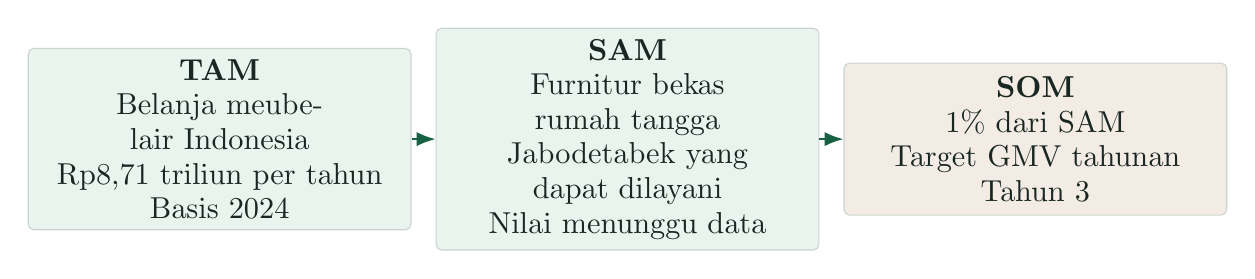
\begin{tikzpicture}[x=1cm,y=1cm]
\node[box,text width=4.58cm,minimum height=1.93cm] (a) at (2.42,0) {\textbf{TAM}\\Belanja meubelair Indonesia\\Rp8,71 triliun per tahun\\Basis 2024};
\node[box,text width=4.58cm,minimum height=1.93cm] (b) at (7.60,0) {\textbf{SAM}\\Furnitur bekas rumah tangga\\Jabodetabek yang dapat dilayani\\Nilai menunggu data};
\node[warmbox,text width=4.58cm,minimum height=1.93cm] (c) at (12.78,0) {\textbf{SOM}\\1\% dari SAM\\Target GMV tahunan\\Tahun 3};
\draw[flow] (a)--(b);\draw[flow] (b)--(c);
\end{tikzpicture}
\end{document}
